% !TEX root = ../paper.tex

\section{Introduction}

Here goes the introduction. We also cite the nice book of Pinedo~\cite{calciu_adaptive_2014,bar-nissan_dynamic_2011,hendler_flat_2010,lotan_skiplist-based_2000,sundell_fast_2003}.

\section{Algorithm X}

Table~\ref{tab:related_algorithms} shows a summary of related algorithms.

\begin{table}[t]
\centering
\captionabove{Related algorithms and their complexity.}
\label{tab:related_algorithms}
\begin{tabular}{ll}
\toprule 
algorithm & complexity \\
\midrule
algorithm Y & $O(n)$ \\
algorithm Z & $O(n \log{n} )$ \\
\bottomrule
\end{tabular}
\end{table}

\section{Evaluation of Algorithm X}

The run-time of our algorithm is shown in Figure~\ref{fig:runtime}.

\begin{figure}[t]
\centering
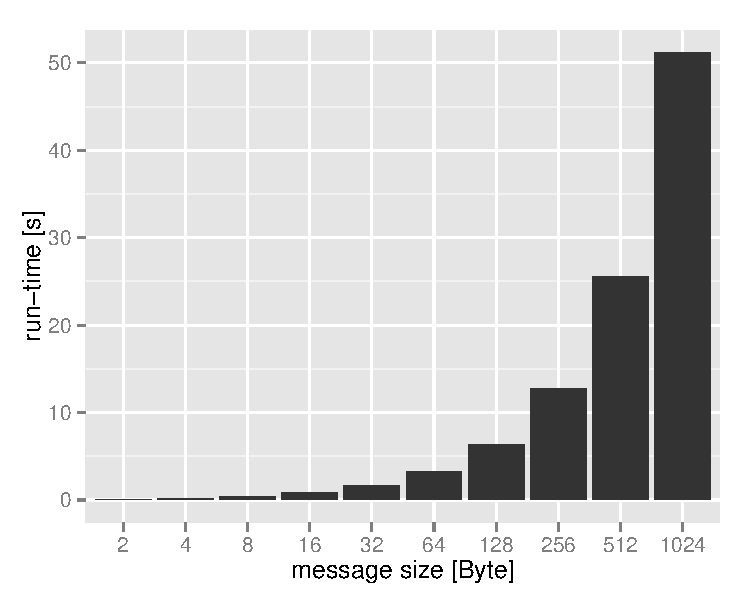
\includegraphics[width=.5\linewidth]{figures/runtime}
\caption{Run-time of algorithm X on machine Y.}
\label{fig:runtime}
\end{figure}

\section{Summary}
We summary the contribution of the papers and this seminar paper.
